\documentclass[border=10pt]{standalone}
\usepackage{tikz}
\usetikzlibrary{arrows.meta, calc, patterns, decorations.pathmorphing}

\begin{document}
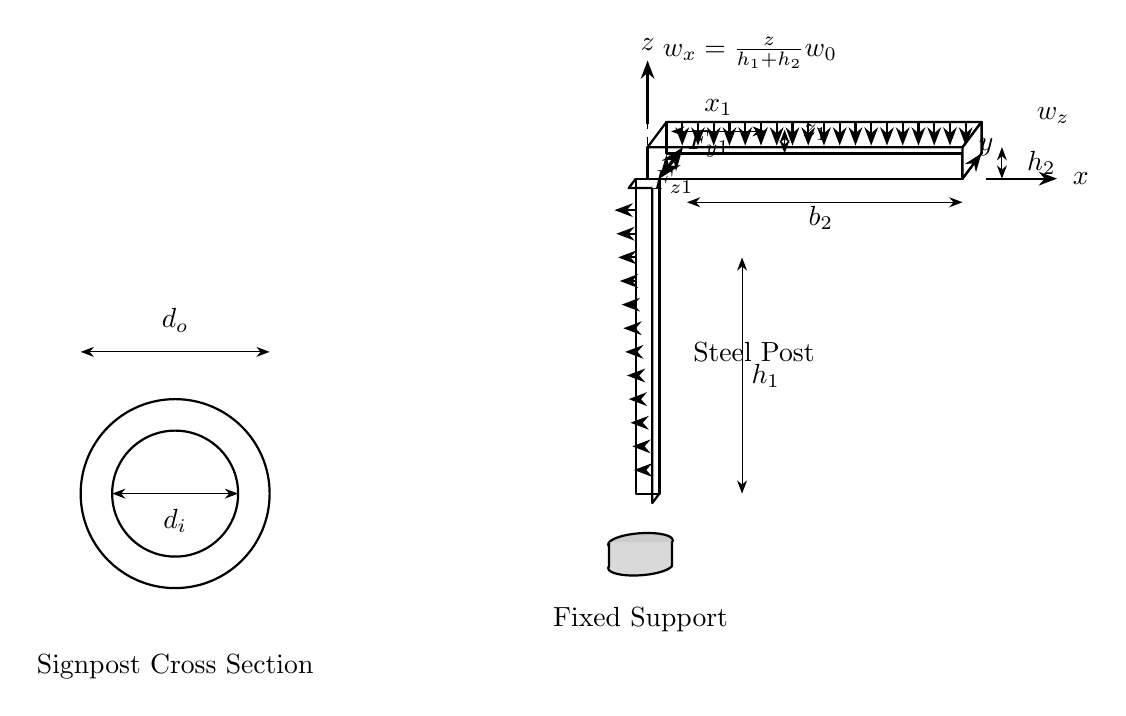
\begin{tikzpicture}[>=Stealth, line join=round]

% Left side - Signpost Cross Section
\begin{scope}[shift={(-6,0)}]
    % Outer circle
    \draw[thick] (0,0) circle (1.2);
    % Inner circle
    \draw[thick] (0,0) circle (0.8);
    
    % Outer diameter arrow
    \draw[<->] (-1.2,1.8) -- (1.2,1.8);
    \node at (0,2.2) {$d_o$};
    
    % Inner diameter arrow
    \draw[<->] (-0.8,0) -- (0.8,0);
    \node at (0,-0.35) {$d_i$};
    
    % Label
    \node[align=center] at (0,-2.2) {Signpost Cross Section};
\end{scope}

% Right side - 3D Structure
\begin{scope}[x={(1cm,0cm)}, y={(0.3cm,0.4cm)}, z={(0cm,1cm)}]
    
    % Fixed support base
    \fill[gray!40] (0,-0.3,-0.5) ellipse (0.4 and 0.3);
    \draw[thick] (0,-0.3,-0.5) ellipse (0.4 and 0.3);
    \draw[thick, fill=gray!30] (-0.4,-0.3,-0.5) -- (-0.4,-0.3,-0.8) 
        arc (180:360:0.4 and 0.3) -- (0.4,-0.3,-0.5);
    
    % Label Fixed Support
    \node[anchor=north] at (0,-0.3,-1.2) {Fixed Support};
    
    % Steel post (vertical)
    \draw[thick, fill=white] (-0.15,0,0) -- (-0.15,0,4) -- (0.15,0,4) -- (0.15,0,0) -- cycle;
    \draw[thick] (0.15,0,0) -- (0.15,-0.3,0) -- (0.15,-0.3,4);
    \draw[thick] (-0.15,0,4) -- (-0.15,-0.3,4) -- (0.15,-0.3,4);
    
    % h1 dimension
    \draw[<->] (1.2,0,0) -- (1.2,0,3);
    \node at (1.5,0,1.5) {$h_1$};
    
    % Horizontal beam
    % Bottom face
    \draw[thick, fill=white] (0,0,4) -- (4,0,4) -- (4,0,4.4) -- (0,0,4.4) -- cycle;
    % Top face
    \draw[thick, fill=white] (0,0.8,4) -- (4,0.8,4) -- (4,0.8,4.4) -- (0,0.8,4.4) -- cycle;
    % Front face
    \draw[thick, fill=white] (4,0,4) -- (4,0.8,4) -- (4,0.8,4.4) -- (4,0,4.4) -- cycle;
    % Side face
    \draw[thick] (0,0,4.4) -- (4,0,4.4) -- (4,0.8,4.4) -- (0,0.8,4.4) -- cycle;
    
    % h2 dimension
    \draw[<->] (4.5,0,4) -- (4.5,0,4.4);
    \node at (5,0,4.2) {$h_2$};
    
    % b2 dimension
    \draw[<->] (0.5,0,3.7) -- (4,0,3.7);
    \node at (2.2,0,3.5) {$b_2$};
    
    % Distributed load on top (wz)
    \foreach \x in {0.2,0.4,...,3.8} {
        \draw[->, thick] (\x,0.8,4.4) -- (\x,0.8,4.1);
    }
    \node at (5,0.5,4.6) {$w_z$};
    
    % Lateral distributed load (wx) - triangular
    \foreach \z in {0.3,0.6,...,3.7} {
        \pgfmathsetmacro{\loadlen}{0.3*\z/4}
        \draw[->, thick] (-0.15,0,\z) -- (-0.15-\loadlen,0,\z);
    }
    
    % Formula for wx
    \node[align=center] at (1,1,5.2) {$w_x = \frac{z}{h_1+h_2}w_0$};
    
    % x1 dimension
    \draw[<->] (0.3,0,4.6) -- (1.5,0,4.6);
    \node at (0.9,0,4.9) {$x_1$};
    
    % z1 dimension
    \draw[<->] (1.5,0.8,4) -- (1.5,0.8,4.3);
    \node at (1.8,1.1,4.15) {$z_1$};
    
    % Forces at connection
    \draw[->, very thick] (0.3,0,4.2) -- (0.3,-0.5,4.2);
    \node at (0.5,-0.6,4.2) {$F_{z1}$};
    
    \draw[->, very thick] (0.3,0,4.2) -- (0.3,0.5,4.2);
    \node at (0.6,0.6,4.2) {$F_{y1}$};
    
    % Coordinate axes
    \draw[->, thick] (0,0,4.7) -- (0,0,5.5);
    \node at (0,0,5.7) {$z$};
    
    \draw[->, thick] (4.3,0,4) -- (5.2,0,4);
    \node at (5.5,0,4) {$x$};
    
    \draw[->, thick] (4,0,4) -- (4,0.8,4);
    \node at (4,1,4) {$y$};
    
    % Dashed reference line
    \draw[dashed] (0,0,4) -- (0,0,4.7);
    \draw[dashed] (0,0,4) -- (0.3,0,4);
    
    % Steel Post label
    \node at (1.5,-0.5,2) {Steel Post};
    
\end{scope}

\end{tikzpicture}
\end{document}